\subsection{Service-Oriented Component Model}

\begin{frame}{iPOJO: A SOCM in Java}
\begin{block}{iPOJO Concepts}
\begin{tabular}{lp{.7\textwidth}}
Component & Instance of a \textit{Factory} class\\
\hline
Factory & (Annotated) Java class, modified by iPOJO after compilation\\
\hline
Handler & Manages a component according to information in its Factory\\
\end{tabular}
\end{block}

\begin{block}{Features}
\begin{itemize}
\item Components are bound by services
\item All the binding and life-cycle management is done by handlers
\item The Factory class only has to provide the business code
\end{itemize}
\end{block}
\end{frame}

\begin{frame}{Component Overview}
\centering
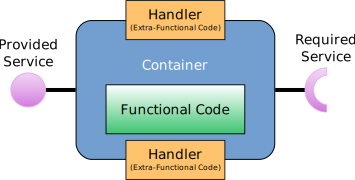
\includegraphics[width=\textwidth]{../imgs/cbse_component}
\end{frame}

\subsection{Code Snippets}

\begin{frame}[fragile]{Snippet: Sample Component}
\begin{block}{Hello world sample}
\begin{minted}{java}
@Component(name="my-factory"}
@Provides(specification=MyInterface.class)
@Instantiate(name="my-instance")
public class MyImplementation implements MyInterface {

	@Requires(optional=true)
	private LogService logger;
	
	public void hello(String name) {
		System.out.println("Hello, " + name + "!");
		logger.log(LogService.LOG_DEBUG,
			"Said hello to " + name);
	}
}
\end{minted}
\end{block}
\end{frame}
